\documentclass[11pt, a4paper]{article}

\usepackage[T1]{fontenc}
\usepackage[utf8]{inputenc}
\usepackage[norsk]{babel}
\usepackage{amsmath}
\usepackage{amsfonts}
\usepackage{amssymb}
\usepackage{graphicx}
\usepackage{verbatim}
\usepackage{caption}
\usepackage{subcaption}
\usepackage{subfig}
\usepackage{float}
\usepackage{program}


\begin{document}
\begin{titlepage}

  \title{\normalsize FYS3150 Computational Physics 2014\\
  \vspace{10mm}
  \huge Oblig 1\\
  \vspace{10mm}
  \normalsize {\bf Løysning av lineære likningar på matriseform.}}

  \author{Øyvind Sigmundson Schøyen}

\end{titlepage}
\maketitle

\begin{figure}[H]
  \centering
  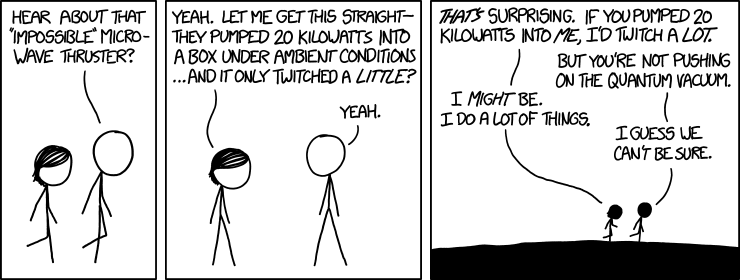
\includegraphics[width=300px]{quantum_vacuum_virtual_plasma.png}
  \caption{xkcd.com/1404/}
\end{figure}

\newpage
  \tableofcontents
\newpage

\section{Introduksjon}
  I dette prosjektet har me tatt for oss ein ein-dimensjonal Poisson likning med Dirichlet randpunkt.
  Me vil simulere ei numerisk løysning på ei andre-ordens differensiallikning.
  Måten me vil gjer dette på er ved å omforme settet med lineære likningar til ei matriselikning. Då 
  kan me bruke radoperasjoner til å lage ei algoritme som gjer det mogleg for oss å løyse 
  likningssettet. Denne matriselikninga vil gje oss ei tridiagonalmatrise $A$ som stort sett består 
  av  nullar. Hensikta er då å sjå at me kan 'kaste' alle nullane og kun behalde elementa frå 
  diagonalane.
  Me vil representere desse som vektorar for å bruke minst mogleg plass. Dette vil og gjere det mogleg  for oss å kunne utføre fleire iterasjoner. Ein vanleg PC vil ikkje kunne klare å representere ei 
  stort større matrise enn $1000\times1000$. Dette fordi han ikkje har stort nok minne. Viss me 
  derimot bruker vektorar vil me kunne ha ei 'matrise' (tre vektorar) som er mykje større. I tillegg 
  vil radreduksjonen gå fleirfoldige mange gonger kjappare.
  Alt av programkode ligg på \texttt{https://github.com/Schoyen/FYS3150/tree/master/Oblig1}


\section{Omforming av differensiallikning til ei matriselikning}
  Me er interesserte i å forme om uttrykket for tilnærminga til den andrederiverte. Me startar med å 
  fjerne brøken. Då får me
  \begin{align*}
    &-\frac{v_{i+1} + v_{i-1} - 2v_i}{h^2} = f_i \\ 
    &\Rightarrow \ \ \ -v_{i+1} + v_{i-1} - 2v_i = h^2f_i = \tilde{b}_i, \ \forall \ i \in [1, n].
  \end{align*}
  Me er no interesserte i å skrive dette om til vektorar og ei matrise. Me kan då skrive det som
  \begin{align*}
    &(2, -1)\cdot(v_1, v_2) = \tilde{b}_1, \\
    &(-1, 2, -1)\cdot(v_1, v_2, v_3) = \tilde{b}_2, \\
    &(-1, 2, -1)\cdot(v_2, v_3, v_4) = \tilde{b}_3, \\
    &\dots \\
    &(-1, 2, -1)\cdot(-v_{i+1}, -v_{i-1}, v_i) = \tilde{b}_i, \\
    &\dots \\
    &(-1, 2)\cdot(v_{n-1}, v_{n}) = \tilde{b}_n.
  \end{align*}
  Det kjem fram frå dette uttrykket at koeffisientane står i ro. Viss me no setter koeffisientane i ei
  matrise vil me kun trenge ein vektor $\mathbf{v}$ beståande av alle $v_i, \ \forall \ i \in [1, n]$
  kor dei vil få dei rette koeffisientane i eit matriseprodukt. Me setter opp matriselikninga.
  \begin{equation*}
    A\mathbf{v} = 
    \begin{pmatrix}
      2 & -1 & 0 & \dots & \dots & 0 \\
      -1 & 2 & -1 & 0 & \dots & \dots \\
      0 & -1 & 2 & -1 & 0 & \dots \\
      \dots & \dots & \dots & \dots & \dots & \dots \\
      0 & \dots & \dots & -1 & 2 & -1 \\
      0 & \dots & \dots & 0 & -1 & 2
    \end{pmatrix}
    \begin{pmatrix}
      v_1 \\
      v_2 \\
      v_3 \\
      \dots \\
      v_{n-1} \\
      v_{n}
    \end{pmatrix} = 
    \begin{pmatrix}
      \tilde{b}_1 \\
      \tilde{b}_2 \\
      \tilde{b}_3 \\       
      \dots \\
      \tilde{b}_{n-1} \\
      \tilde{b}_n
    \end{pmatrix} = \mathbf{\tilde{b}}
  \end{equation*}
  Eit matriseprodukt av dette uttrykket vil gje oss
  \begin{align*}
    &2v_1 - v_2 = \tilde{b}_1 \\
    &-v_1 + 2v_2 - v_3 = \tilde{b}_2 \\
    &\dots \\
    &-v_{i-1} + 2v_i - v_{i+1} = \tilde{b}_i \\
    &\dots \\
    &-v_{n-2} + 2v_{n-1} -v_{n} = \tilde{b}_{n-1} \\
    &-v_{n-1} + 2v_{n} = \tilde{b}_n.
  \end{align*}
  Dette fordi koeffisientane er omringa av nullar som automatisk vil fjerne resten av ledda frå 
  $\mathbf{v}$.

  \subsection{Utleiing av eksakt løysning}
    For å sjå at den eksakte løysninga er riktig treng me berre å derivere uttrykket to gonger for å
    sjå at det vert det same som uttrykket til $f$.
    \begin{align*}
      &u(x) = 1 - x - xe^{-10} - e^{-10x}, \\
      &\frac{du(x)}{dx} = -1 -e^{-10} + 10e^{-10x}, \\
      &\frac{d^2u(x)}{dx^2} = -100e^{-10x} = f(x).
    \end{align*}

\newpage

\section{Algoritma}
  For å løyse ei matriselikning bruker me radoperasjoner på matrisa. Desse vil igjen bli utførde på
  løysningsvektoren (her kalla $\mathbf{\tilde{b}}$). Målet med likninga er å omforme matrisa til ei 
  spesiell øvre-  og nedrematrise som me kan løyse. 
  
  \subsection{Dekomponering}
    I den fyrste matrisa vil me fjerne alle verdiar over diagonalen slik at me står igjen med 
    $\lambda_i$ og $a_i, \ \forall \ i \in [1, n]$. I den andre vil me kun ha einarar på 
    diagonalen og $\gamma_i, \ \forall \ i \in [1, n - 1]$ over.

    \begin{align*}
      &A =
      \begin{pmatrix}
        b_1 & c_1 & \dots & \dots & \dots & \dots \\
        a_2 & b_2 & c_2 & \dots & \dots & \dots \\
        \dots & a_3 & b_3 & c_3 & \dots & \dots \\
        \dots & \dots & \dots & \dots & \dots & \dots \\
        \dots & \dots & \dots & a_{n-1} & b_{n-1} & c_{n-1} \\
        \dots & \dots & \dots & \dots & a_n & b_n
      \end{pmatrix} = LU\\
      &=
      \begin{pmatrix}
        \lambda_1 & \dots & \dots & \dots & \dots & \dots \\
        a_2 & \lambda_2 & \dots & \dots & \dots & \dots \\
        \dots & a_3 & \lambda_3 & \dots & \dots & \dots \\
        \dots & \dots & \dots & \dots & \dots & \dots \\
        \dots & \dots & \dots & a_{n-1} & \lambda_{n-1} & \dots \\
        \dots & \dots & \dots & \dots & a_n & \lambda_n 
      \end{pmatrix}
      \begin{pmatrix}
        1 & \gamma_1  & \dots & \dots & \dots & \dots \\
        \dots & 1 & \lambda_2 & \dots & \dots & \dots \\
        \dots & \dots & 1 & \gamma_3 & \dots & \dots \\
        \dots & \dots & \dots & \dots & \dots & \dots \\
        \dots & \dots & \dots & \dots & 1 & \gamma_{n-1} \\
        \dots & \dots & \dots & \dots & \dots & 1 
      \end{pmatrix}.
    \end{align*}
    Multiplikasjon av matrisene $LU$ vil gje oss $A$. Me bruker dette til å finne eit uttrykk for 
    $\gamma_i, \ \forall \ i \in [1, n-1]$ og $\lambda_i, \ \forall \ i \ \in [1, n]$. Det vil gje oss
    \begin{align*}
      &\lambda_1 = b_1, \qquad \gamma_1 = \frac{c_1}{\lambda_1}, \\
      &\lambda_2 = b_2 - a_2\gamma_1, \qquad \gamma_2 = \frac{c_2}{\lambda_2} \\ 
      &\dots \\
      &\lambda_i = b_i - a_i\gamma_{i-1}, \qquad \gamma_i = \frac{c_i}{\lambda_{i}}, \\
      &\dots \\
      &\lambda_n = b_n - a_n\gamma_{n-1}, \qquad \gamma_n = \frac{c_n}{\lambda_n}.
    \end{align*}

  \subsection{Forward Substitution}
    No gjenstår det å løyse likningane $L\mathbf{y} = \mathbf{\tilde{b}}$ og $U\mathbf{v} =
    \mathbf{y}$. I programmet vil dette bli gjort litt annleis. Der vil me løyse $L\mathbf{v} 
    = \mathbf{\tilde{b}}$ og $U\mathbf{v} = \mathbf{v}$. Dette for å spare plass i minnet, men det 
    kjem me til. Likninga $L\mathbf{y} = \mathbf{\tilde{b}}$ vil gje oss likningssetta under.
    
    \begin{align*}
      \lambda_1y_1 = \tilde{b}_1 \qquad &\Rightarrow \qquad y_1 = \frac{\tilde{b}_1}{\lambda_1}, \\
      a_2y_1 + \lambda_2y_2 = \tilde{b}_2 \qquad &\Rightarrow \qquad y_2 = \frac{\tilde{b}_2 - a_2
      y_1}{\lambda_2}, \\
      &\dots \\
      a_iy_{i-1} + \lambda_iy_i = \tilde{b}_i \qquad &\Rightarrow \qquad y_i = \frac{\tilde{b}_i
      - a_iy_{i-1}}{\lambda_i}, \\
      &\dots \\
      a_ny_{n-1} + \lambda_ny_n = \tilde{b}_n \qquad &\Rightarrow \qquad y_n = \frac{\tilde{b}_n
      - a_ny_{n-1}}{\lambda_n}.
    \end{align*}

  \subsection{Backward Substitution}
    Til slutt bruker me backward substitution til å finne den endelege løysninga. Me må då løyse
    likninga $U\mathbf{v} = \mathbf{y}$. Denne likninga må me løyse baklengs. Me får

    \begin{align*}
      v_n &= y_n, \\
      v_{n-1} + \gamma_{n-1}v_n = y_{n-1} \qquad &\Rightarrow \qquad v_{n-1} = y_{n-1} - 
      \gamma_{n-1}v_n, \\
      &\dots \\
      v_i + \gamma_iv_{n+1} = y_i \qquad &\Rightarrow \qquad v_i = y_i - \gamma_iv_{i+1}, \\
      &\dots \\
      v_1 + \gamma_1v_2 = y_1 \qquad &\Rightarrow \qquad v_1 = y_1 - \gamma_1v_2.
    \end{align*}

  \subsection{Antal FLOPS}
    For å finne ut kor mange flyttalsoperasjoner (FLOPS) me treng kan me telje kor mange 
    aritmetiske operasjoner me gjer per iterasjon. I løkka (eg har ikkje rekna med startverdiar og 
    dei fyrste operasjonane utanfor løkka) har me 6 FLOPS i Forward Substitutionen (eg har her 
    rekna divisjon som ein FLOP) medan me i Backward Substitutionen har 2 FLOPS. Det gjer oss 8 FLOPS 
    per iterasjon og totalt $8n$ FLOPS, kor $n$ er antal iterasjoner.


  \subsection{Køyretid}
    Idet ein køyrer programmet \texttt{Plotter.py} vil me få ut køyretidene (tida er kun tatt frå
    for-løkka i programmet).
    \verbatiminput{utskrift.txt} \
    Desse køyretidene vil variere veldig med dagsformen til pc'en som køyrer programmet samt
    hardwaren pc'en i seg sjølv. Hovudpoenget er å sjå skjelnaden på dei to algoritmane.
    Køyretiden er gjeve ved $\mathcal{O}(8n)$.


\newpage

\section{Programma}
  Alle algoritmar og tung utrekning vert gjennomført i C++. Programmet skriv ut resultata til fil,
  kor desse vert henta av eit program i Python som plottar resultata. Sjølve køyringa av programmet 
  vert styrt i Python. Ein treng difor kun å køyre programmet \texttt{Plotter.py} for å få ut all
  informasjon. 

  \subsection{\texttt{Plotter.py}}
    Python-programmet står for sjølve gjennomføringa av heile prosjektet. Eit kall på 
    programmet køyrer C++ programmet for forskjellige verdiar av $n$ samt dei forskjellige
    metodane. C++ skriv ut resultata til filer som Python tar imot. Python les verdiane og lagrar dei
    i arrays i klassa Plotter. Desse vert deretter plotta.
   
  \subsection{\texttt{Project1.cpp}}
    C++-programmet tek imot $n$-verdiar og kva løysningsmetode som skal nyttast frå kommandolinja.
    Algoritmane vert implementerte i eigne funksjonar.

    \begin{program}
      \COMMENT{Startverdier for TDMA-algoritma}
      \lambda_1 = b_1
      v_1 = \frac{\tilde{b}_1}{\lambda_1}
      \gamma_1 = \frac{c_1}{\lambda_1}
      \COMMENT{Forward sweep}
      \FOR i = 2 \TO i < n+1 \STEP 1
        \lambda_i = b_i - \gamma_{i-1}a_i
        \gamma_i = \frac{c_i}{\lambda_i}
        v_i = \frac{\tilde{b}_i - a_iv_{i-1}}{\lambda_i}
        \OD
      \COMMENT{Backward sweep}
      \FOR i = n \TO i > 0 \STEP -1
      v_i = \gamma_iv_{i+1} - v_i
      \OD
    \end{program}
    \begin{program}
      \COMMENT{Startverdiar for LU-algoritma frå Armadillo-biblioteket}
      lu(L, U, P, A) 
      \COMMENT{Forward sweep}
      \FOR i = 1 \TO i < n+1 \STEP 1
      y_i = \tilde{b}_i
      \FOR j = 1 \TO j < i \STEP 1
        y_i = L_{i-1, j-1}y_j - y_i
        \OD
      y_i = \frac{L_{i-1, i-1}}{y_i}
      \OD
      \COMMENT{Backward sweep}
      \FOR i = n \TO i > 0 \STEP -1
        v_i = y_i
        \FOR j = i+1 \TO j < n+1 \STEP 1
          v_i = U_{i-1, j-1}v_j - v_i
          \OD
        v_i = \frac{U_{i-1, i-1}}{v_i}
        \OD
    \end{program}

    

\newpage

\section{Resultat}
  Metoden som vert nytta til å løyse likningssettet er veldig sterk. Allerede for $n = 100$ vil 
  den numeriske løysninga ligge heilt på den eksakte løysninga. 

  \subsection{Plott over løysningar}

    \begin{figure}[H]
      \centering
      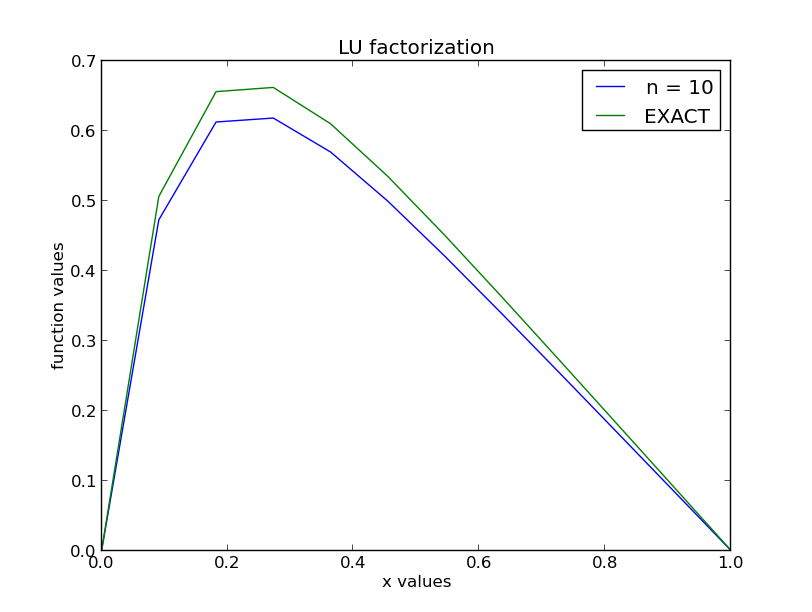
\includegraphics[width=300px]{LU10.png} \\
      \caption{LU for $n = 10$}
    \end{figure}
    \begin{figure}[H]
      \centering
      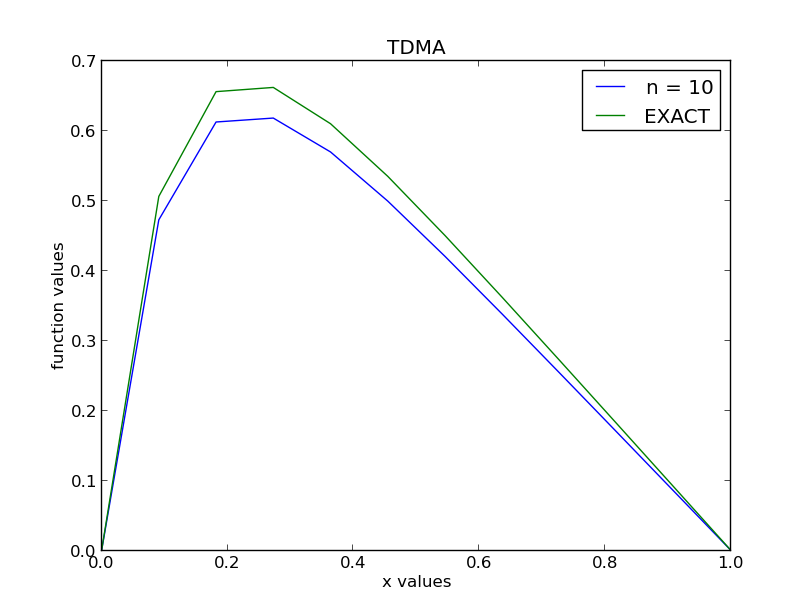
\includegraphics[width=300px]{TDMA10.png} \\
      \caption{TDMA for $n = 10$}
    \end{figure}

    Me kan sjå at løysninga for $n = 10$ er langt i frå eksakt foreløpig.

    \begin{figure}[H]
      \centering
      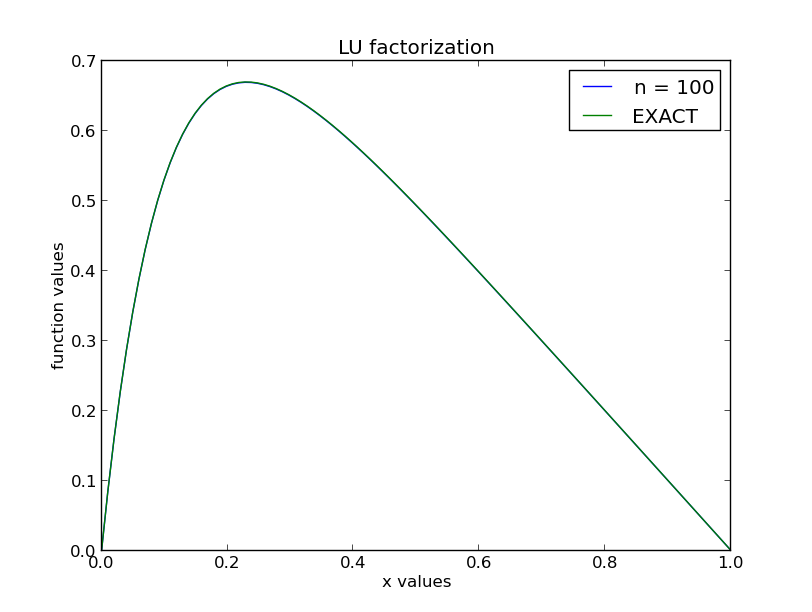
\includegraphics[width=300px]{LU100.png} \\
      \caption{LU for $n = 100$}
    \end{figure}
    \begin{figure}[H]
      \centering
      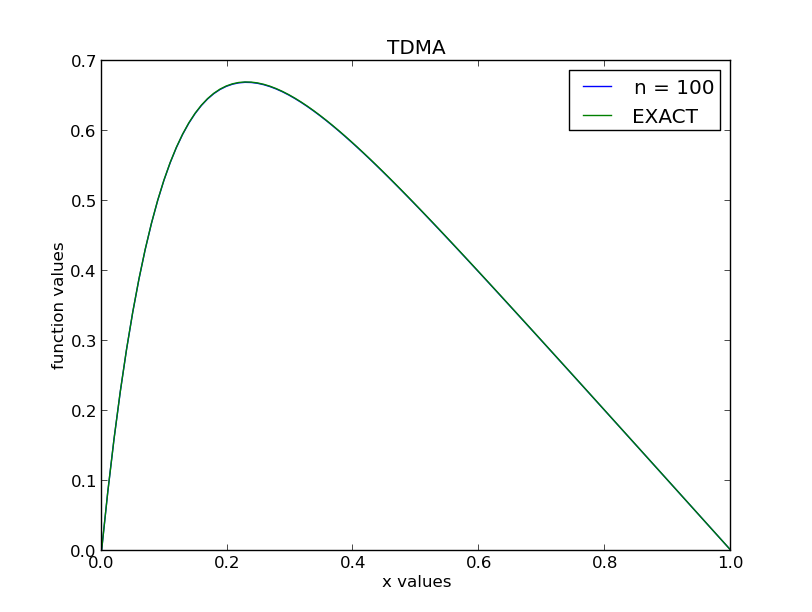
\includegraphics[width=300px]{TDMA100.png} \\
      \caption{TDMA for $n = 100$}
    \end{figure}

    Dei resterande plotta vil bli heilt like då den numeriske løysninga ligg heilt på den 
    eksakte løysninga.

\newpage
  \subsection{Feilestimat}
    Grafen til feilestimatet gjer oss ei tilnærma lineær nedgang. For $n = 1000000$ derimot skjer 
    det noko underleg. Plutseleg stig feilen igjen. 

    \begin{figure}[H]
      \centering
      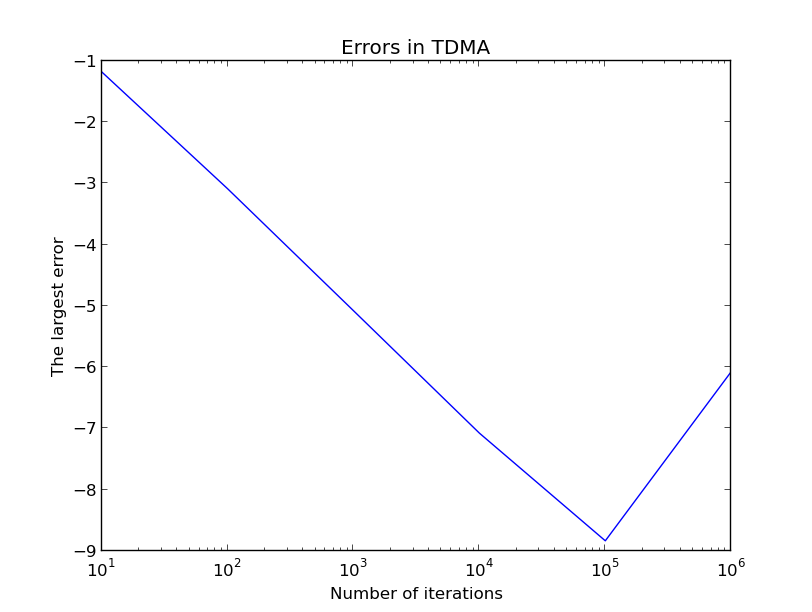
\includegraphics[width=300px]{ERROR.png} \\
      \caption{Feilestimat}
    \end{figure}

    Dette skjer fordi numerisk avrunding slår inn. PC'en klarer berre å håndtere eit visst antal
    signifikante tal. Når talet overskrid denne grensa vil numerisk avrunding slå inn og feilen vil
    stige.

    \begin{center}
      \begin{tabular}{|l||r|}
        \hline
        Antal iterasjoner & Feil \\
        \hline
        \input{utskrift2.txt}
        \hline
      \end{tabular}
    \end{center}

    Det siste leddet viser korleis feilen vil stige etterkvart som me auker antal iterasjoner.

\end{document}
